
% This is a LaTeX Beamer for our project presentation

\documentclass{beamer}
\usetheme{Madrid}
\usecolortheme{default}
\usepackage[french]{babel}
\usepackage[utf8]{inputenc}
\usepackage{amsmath, amssymb}
\usepackage{subcaption}
\usepackage{listings}

\title{Projet ncpol3sdpa}
\subtitle{Audit de Présentation}
\author{Alain, Mathis, Nazar, Thomas, Yann}
\date{\today}

\begin{document}

\begin{frame}
\titlepage
\end{frame}

\begin{frame}{Sommaire}
\tableofcontents
\end{frame}

\section{Présentation du Problème}

\begin{frame}{Présentation du Problème}
\begin{itemize}
    \item Développement d'une bibliothèque Python pour l'optimisation polynomiale: \textbf{ncpol3sdpa}
    \item Successeur de \textbf{ncpol2sdpa}
    \item Outil pour calculer des approximations aux problèmes d'optimisation polynomiale
\end{itemize}
\end{frame}

\begin{frame}{Contexte Mathématique}
L'optimisation polynomiale cherche à résoudre des problèmes de la forme :
\begin{align}
\max_{x_1, \ldots, x_n} &\quad f(x_1, \ldots, x_n) \\
\text{s.t.} &\quad g_i(x_1, \ldots, x_n) \leq 0 \quad \forall i
\end{align}

où $f,g_i \in \mathbb{K} [x_1,\ldots,x_n]$.
\vspace{0.5cm}

\begin{itemize}
    \item Problèmes NP-difficiles
    \item Approchés par des techniques d'optimisation convexe
    \item Basés sur les matrices de moments et polynômes sommes de carrés
\end{itemize}
\end{frame}

\section{Enjeux et Objectifs}

\begin{frame}{Enjeux et Objectifs}
Notre bibliothèque vise à :
\begin{enumerate}
    \item \textbf{Moderniser l'approche} : Créer une version plus flexible et efficace que ncpol2sdpa
    \item \textbf{Améliorer les performances} : Optimiser les calculs pour des problèmes complexes
    \item \textbf{Utiliser plusieurs solvers} : Intégrer différents solveurs pour élargir les possibilités de résolution
\end{enumerate}
\end{frame}

\section{Notre Équipe}

\begin{frame}{Notre Équipe}
\begin{description}
    \item[Alain]: problème maxcut
    \item[Mathis]: polynômes complexes et non commutatifs
    \item[Nazar]: tests et intégration continue
    \item[Thomas]: SOS decomposition
    \item[Yann]: organisation technique
\end{description}
\end{frame}

\begin{frame}{SOS decomposition}

    La décomposition sum ofsSquare : 
$$f(x) - \lambda = SOS(x) - \sum_i SOS_i(x) g_i(x)$$
Avec $SOS_i(x) = \sum_k p_k(x)^2$  
\end{frame}

\section{Organisation du Travail}

% \begin{frame}{Organisation du code}

% \begin{text}
% ncpol3sdpa/
% ├── __init__.py
% └── utils/
% \end{text}

% \end{frame}

\begin{frame}{Répartition des Tâches}
Nous avons organisé notre travail en modules distincts :
\begin{itemize}
    \item Implémentation du noyau mathématique
    \item Tests et validation
    \item Documentation et exemples d'utilisation
\end{itemize}
\end{frame}

\begin{frame}{Méthodologie}
\begin{itemize}
    \item \textbf{Développement par branche} : Chaque membre travaille sur une branche dédiée. Les branches sont fusionnées toutes les deux semaines.
    \item \textbf{Revues de code} systématiques avant intégration
    \item \textbf{Tests unitaires} et intégration continue
    \item \textbf{Réunions bimensuelles} avec notre superviseur (Peter Brown)
\end{itemize}
\end{frame}

\begin{frame}{Planning - Objectifs fin P3}

% \begin{center}
% \textbf{Objectifs fin P3}
% \end{center}
Cas d'optimisation des polynômes commutatifs et réels
\begin{itemize}
    \item[\checkmark] Partie "Algèbre", manipulation symbolique des polynômes
    \item[\checkmark] Construction de la matrice des moments de la hiérarchie de Lasserre
    \item[\checkmark] Communication avec des solveurs de SDP
\end{itemize}
\end{frame}

\begin{frame}{Planning - Objectifs fin P4}

% \begin{center}
% \textbf{Objectifs fin P4}
% \end{center}
\begin{itemize}
    \item[$\square$] Documentation, tutoriel et exemples
    \item[\checkmark] Jeux de tests (CI/CD)
    \item[\checkmark] Cas de polynômes complexes
    \item[$\square$] Cas de polynômes non commutatifs
    \item[$\square$] Optimisations pour améliorer les performances
\end{itemize}
\end{frame}

\section{Applications et Impact}

\begin{frame}{Applications et Impact}
\begin{itemize}
    \item Utilisable en informatique quantique
    \item Résolution de problèmes d'optimisation
    \item \texttt{ncpol2sdpa} est actuellement utilisée par des chercheurs
\end{itemize}
\end{frame}

\begin{frame}{Applications}

\begin{itemize}
    \item Problème maxcut
    \item Ferme à mob dans Minecraft
\end{itemize}

\begin{figure}
    \centering
    \begin{subfigure}{0.4\textwidth}
        \centering
        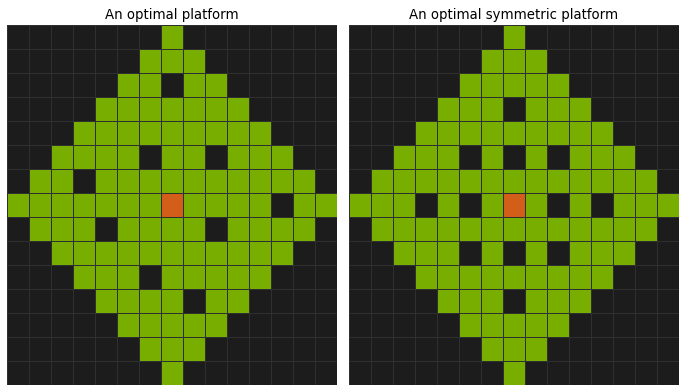
\includegraphics[width=\textwidth]{img/minecraft-mob-farm.png}
        \caption{Exemple d'application : optimisation dans Minecraft}
    \end{subfigure}
    % \hfill
    \begin{subfigure}{0.4\textwidth}
        \centering
        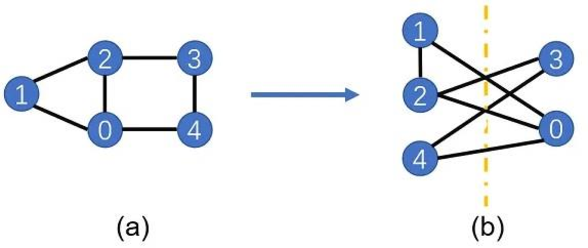
\includegraphics[width=\textwidth]{img/maxcut.png}
        \caption{Exemple d'application : optimisation du problème maxcut}
    \end{subfigure}
\end{figure}

\end{frame}

\begin{frame}{Merci de votre attention}
\begin{center}
    {\Large Place aux questions}
\end{center}
\end{frame}

\end{document}